
\documentclass[smallextended]{svjour3} 

% graphicx was written by David Carlisle and Sebastian Rahtz. It is
% required if you want graphics, photos, etc. graphicx.sty is already
% installed on most LaTeX systems. The latest version and documentation can
% be obtained at: 
% http://www.ctan.org/tex-archive/macros/latex/required/graphics/
% Another good source of documentation is "Using Imported Graphics in
% LaTeX2e" by Keith Reckdahl which can be found as epslatex.ps or
% epslatex.pdf at: http://www.ctan.org/tex-archive/info/
%
% latex, and pdflatex in dvi mode, support graphics in encapsulated
% postscript (.eps) format. pdflatex in pdf mode supports graphics
% in .pdf, .jpeg, .png and .mps (metapost) formats. Users should ensure
% that all non-photo figures use a vector format (.eps, .pdf, .mps) and
% not a bitmapped formats (.jpeg, .png). IEEE frowns on bitmapped formats
% which can result in "jaggedy"/blurry rendering of lines and letters as
% well as large increases in file sizes.
%
% You can find documentation about the pdfTeX application at:
% http://www.tug.org/applications/pdftex

\usepackage[draft]{comments}
\usepackage{tikz}
\usepackage{pgfplots}
\pgfplotsset{compat=1.3}
\usepackage{graphicx, epsfig}
\usepackage{xspace}  %% Package used for the \NB{} abbreviation
\usepackage{algorithm}
\usepackage{algpseudocode}
\usepackage{color}
\usepackage{url}
\usepackage{hyperref}
\usepackage{listings}
\usepackage{tikz}% http://ctan.org/pkg/pgf
\usetikzlibrary{calc}
\usepackage{amssymb,amsmath}

\newcommand{\cbcomment}[1]{\comment{CB}{#1}}
\newcommand{\khcomment}[1]{\comment{KH}{#1}}
\newcommand{\vjcomment}[1]{\comment{VJ}{#1}}
\newcommand{\jmcomment}[1]{\comment{JM}{#1}}
\newcommand{\mgcomment}[1]{\comment{MG}{#1}}

% http://tex.stackexchange.com/questions/1559/adding-a-large-brace-next-to-a-body-of-text/1570#1570
\newcommand{\tikzmark}[1]{\tikz[overlay,remember picture] \node (#1) {};}

\lstset{
numbers=left,
numbersep=5pt,
numberstyle=\color{gray}
%    frame=single,
%    mathescape % Allows escaping to (La)TeX mode within $..$
}


% correct bad hyphenation here
\hyphenation{op-tical net-works semi-conduc-tor}


\begin{document}
	
	\title{Programming Heterogeneous Parallel Machines using Refactoring and Monte-Carlo Tree Search}
	
	
	\author{Christopher Brown         \and
		Vladimir Janjic  \and 
		M. Goli \and
		J. McCall 
	}
	
	%\authorrunning{Short form of author list} % if too long for running head
	
	\institute{C. Brown, V. Janjic \at
		School of Computer Science, University of St Andrews, UK. \\
		\email{cmb21,vj32@st-andrews.ac.uk}           %  \\
		%             \emph{Present address:} of F. Author  %  if needed
		\and
		M. Goli, J. McCall \at
		Robert Gordon University, Aberdeen, UK. \\
		\email{m.goli1, j.mccall@rgu.ac.uk}
	}

\date{Received: date / Accepted: date}

%\author{\IEEEauthorblockN{Christopher Brown\IEEEauthorrefmark{1}, Vladimir Janjic\IEEEauthorrefmark{1}, Kevin Hammond\IEEEauthorrefmark{1}}
%\IEEEauthorblockA{\IEEEauthorrefmark{1}School of Computer Science\\
% University of St Andrews\\
% St Andrews\\
% United Kingdom\\E-Mail : \{cmb21,jv32,kh8\}@st-andrews.ac.uk}
%University of St Andrews, St Andrews, UK\\E-Mail : \{cmb21,jv32,kh8\}@st-andrews.ac.uk}
%\and
%\IEEEauthorblockN{Mehdi Goli\IEEEauthorrefmark{2}, John McCall\IEEEauthorrefmark{2}}
%\IEEEauthorblockA{\IEEEauthorrefmark{2}School of Computer Science\\
%Robert Gordon University,
%Aberdeen, UK
%\\E-Mail : \{m.goli1,j.mccall\}@rgu.ac.uk}}

% make the title area
\maketitle


\begin{abstract}
Heterogeneous shared-memory systems, comprising a mixture of CPUs
and GPUs, are increasingly common. 
%% Definitely not mainstream.
%  becoming mainstream for parallel programming. 
Current techniques for programming such systems (such as OpenCL
or CUDA+OpenMP) offer very little abstraction, however, relying on the programmer to deal with
many low-level details such as thread creation, data
transfers, scheduling etc. An even bigger problem is that the division
of work between CPUs and GPUs needs to be performed manually by the programmer.
In this paper we describe a new technique for programming heterogeneous
systems using a combination of
programmer-directed \emph{refactoring} % (built on top of algorithmic skeletons) 
and \emph{Monte Carlo Tree Search (MCTS)}. Refactoring eases the task of
writing parallel programs by offering the programmer step-by-step
guidance for transforming theier sequential program into an equivalent parallel
program, and/or for transforming parallel programs into better ones. The MCTS algorithm enables us to derive good
mappings of the resulting parallel programs to the available heterogeneous hardware.
We demonstrate the applicability of our methodology using an Image
Convolution benchmark, obtaining a speedup of 40.91
on a machine comprising 2x 2.4Ghz 12-core AMD Opteron 6176 CPUs coupled an NVidia Tesla C2050 with 448 GPU
cores running at 1.16GHz.
% -core machine with a GPU . 
We also demonstrate that the speedups that we obtain using
the mappings that the MCTS algorithm suggests are within 5\% of
the best possible speedups that can be obtained. %  for the particular application.
\end{abstract}

% For peer review papers, you can put extra information on the cover
% page as needed:
% \ifCLASSOPTIONpeerreview
% \begin{center} \bfseries EDICS Category: 3-BBND \end{center}
% \fi
%
% For peerreview papers, this IEEEtran command inserts a page break and
% creates the second title. It will be ignored for other modes.
%\IEEEpeerreviewmaketitle



\section{Introduction}
\noindent
Heterogeneous multicore systems, comprising mixtures of
CPUs and GPUs, are increasingly common, combining perhaps
dozens of CPU cores with perhaps hundreds of GPU cores.
% Devices such as Intel's recently announced 60-core Xeon Phi co-processor open the possibility of even larger scale parallelism.
Programming such systems remains difficult, however.
% , are rapidly becoming mainstream devices for parallel
% programming, offering a huge amount of potential processing power. 
% Intel's latest announcement of the new
% 60-core Xeon Phi co-processor further exasperates the situation, leading to a \emph{parallel programming crisis}:
% most applications programmers simply lack the expertise in parallelism, where knowing when and where to effectively deploy parallelism
% seems an almost impossibility. 
State-of-the-art programming techniques, such as OpenCL or \\ CUDA+OpenMP,
%  generally falls into two camps: % , forming a dangerous dichotomy:
generally involve exploiting low-level programming techniques that
require precise in-depth knowledge of the GPU architecture together with
information about data-transfers, scheduling decisions etc., usually do not scale easily or well, and cannot easily
be retargeted to alternative hardware architectures.
% VJ : I would remove this:
%  (indeed, an applications programmer wouldn't be expected to implement
% an OS every time he/she writes an application)
%% Not the only approach. KH
% or, high-level approaches, using skeletons,
% that abstract away the low-level complexities but present new challenges, such as understanding when and where to effectively
% deploy which skeleton, and which (if any) tuning parameters to deploy.
%
In this paper, we introduce a new technique for programming heterogenous parallel systems,
based on a combination of high-level parallel patterns, % skeletons, 
template-based implementations (skeletons),
advanced refactoring technology, and a new static mapping approach that
exploits Monte Carlo Tree Search (MCTS) to find good mappings of tasks to
heterogeneous architectures. %  based model for static mapping.
Parallel patterns provide design-time \emph{choice} and parallel program \emph{structure};
% parallelism; 
skeletons provide correspondingly structured implementations and a decomposition into parallel program
components; 
the MCTS-based mapping model provides
the programmer with \emph{decisions} that ensure good static mappings
of these components to the available heterogeneous hardware; 
and refactoring provides the \emph{discipline} and \emph{tool-support} to introduce and tune the
parallelism, abstracting over the detail of the skeletons, and exposing performance information
based on the decisions provided by the static mapping.
% VJ : I would move part (or all of the) text below to the refactoring section
%Unlike automated parallelisation techniques, which works only under specific conditions, and for a limited set of examples, refactoring
%takes a more structured semi-automatic approach, aimed at increasing
%programmability and intuition for building and tuning parallel
%programs. 
% Also, unlike automatic parallelisation, refactoring can support the intelligent programmer (whether experienced or inexperienced), by fitting into their natural software engineering cycle, supporting their decisions and guiding them down the correct paths: refactorings can \emph{warn} the user if they are doing something wrong; give \emph{guidance} to the programmer to choose the best skeleton or tuning configuration; or, \emph{switch} between different underlying skeleton models/implementations.
%
We demonstrate our technique on an Image Convolution
benchmark, targeting a 24-core machine, comprising 2x 2.4Ghz 12-core AMD Opteron 6176 CPUs,
plus an NVidia Tesla C2050 GPU with 488 1.16GHz cores.
Using this machine, we obtain
% VJ : whatever 'easy speedup' is supposed to mean
scalable speedups of up to 40.91 over the sequential implementation.
Our results show that these speedups are within 5\% of the best possible speedup using any possible static mapping.
%  and the accuracy
% % VJ : accuracy is not really a word for this
%  of the static mappings estimated by the MCTS-based model. 
% VJ : Tesla GPU really doesn't say anything. We need to either say
% how many cores does the GPU has, or to just say 'with a GPU'
% In order to demonstrate the principles of our approach, we limit our methodology
% to
Our concrete experiments are conducted using C++ and the FastFlow skeleton library. 
However, the principles and techniques that we
describe are not limited to C++ or FastFlow, but are \emph{completely generic}, and can easily be
transferred to other languages/paradigms, such as C, Java, Fortran or Haskell;
to other skeleton libraries, such as SkePU; 
and to other parallel implementations, such as direct CUDA, pThreads or Cilk.
% VJ : these are not really skeleton implementations
%  (such as Pthreads/OpenMP/Cilk).

\begin{figure*}[t]
\begin{center}
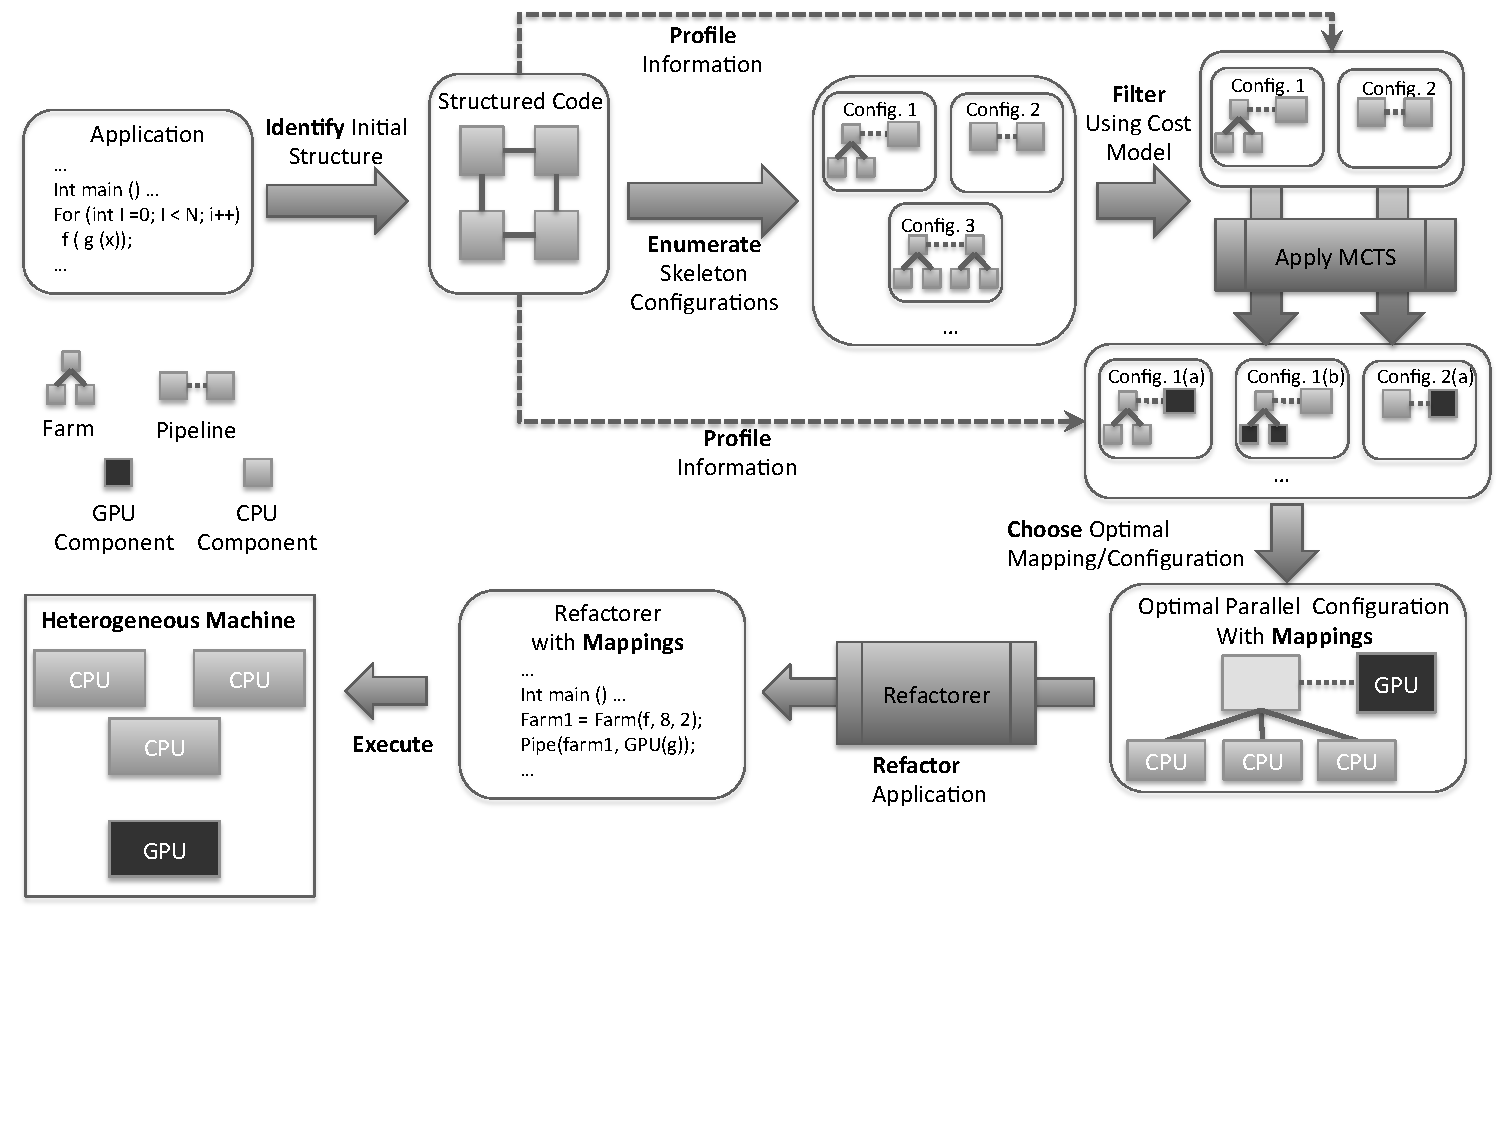
\includegraphics[width=0.99\linewidth]{figures/methodology.pdf}
\caption{Overview of our technique.  We start with a (sequential)
  program with an identified skeletal structure. All configurations of the
  structure are then enumerated, and can be filtered using cost
  models. The remaining configurations are given to a Monte-Carlo Tree
  Search algorithm, which determines mapping and skeletal parameters. 
  This information is then given to a
  refactoring tool, which semi-automatically applies the skeletal
  transformation. } % , under guidance from the programmer.}
\label{overview}
\end{center}
\end{figure*}

The paper makes the following research contributions:
% \vspace{-12pt}
\begin{enumerate}
\item we introduce a new technique for building
  parallel programs, based on parallel patterns, semi-automatic refactoring, and high-level algorithmic skeletons;
\item we introduce a new static-mapping framework, based on Monte-Carlo Tree Search simulations, for deriving
  efficient mappings of parallel application threads to heterogeneous CPU
  and GPU hardware;
% VJ : This is not such a major contribution, if you ask me
%\item We define a precise specification for the static mapping problem; and,
% VJ : Since these refactorings are still manual, I would say that the
% static mapping stuff is a bigger contribution%
%\item 
%We introduce a number of novel refactorings for introducing parallelism for heterogenous many-core systems, implemented in the CDT refactoring plugin for Eclipse;
\item 
we show how our technique applies to a convolution benchmark,
  obtaining promising and scalable speedups on a heterogeneous parallel
  system.
\end{enumerate}

\section{A Technique for Programming Hetereogeneous Parallel Machines} \label{sec:methodology}
% VJ : I would remove this. I think our technology is aimed also at
% good parallel programmers. Besides, we cannot really expect the
% inexperienced parallel programmer to provide us with good
% decomposition of a problem, good CPU and GPU implementations of
% functions etc.
% Our methodology is aimed at inexperienced parallel programmers who lack the experience 
% or expertise in deploying parallelism in their applications, particularly for heterogeneous systems.
\noindent
Our general technique is shown in Figure \ref{overview}.  We assume that the initial application
is already in a ``hygienic'' state, i.e., that the
%  the algorithmic structure has been clearly defined and that the 
units of computation are defined as \emph{components} whose dependencies and interactions are clearly specified.
% VJ : I am not sure about below  
%% That's the key point...
% that do not contain side-effects nor dependencies with other
% components. 
We also assume that CPU and GPU implementations are available for each component, in a way that allows them
to be linked (perhaps using automatically provided marshalling/unmarshalling code, where it is necessary to
offload a component); and that profiling information is also available.
%% PROGRAMMER, NOT USER!!
% The user also supplies, upfront the CPU and/or GPU implementation for each component (where appropriate)
% and also the profiling results for the components.
\begin{enumerate}
\item Assuming that we start with a program that has not previously been parallelised, 
  it is first necessary to
% he user starts with their program, where they then
  \emph{identify} and extract the algorithmic structure in the form of an
  abstract \emph{skeletal configuration}, which encapsulates the
  structure of the algorithm together with its component information,
  showing the relationships and dependencies between the components,
  and eliminating/exposing any shared state through interfaces to the component.
%   and exposing an interface to the component in the form of input/outputs.
\item Given the identified skeletal configuration, all possible
  equivalent skeletal configurations of the program are \emph{enumerated} up to
  a given depth of nesting, resulting in a number of possible parallel \emph{factorisations}.
\item Using \emph{profiling} information, these factorisations are \emph{filtered} using a cost model, if desired,
  to restrict the number of possibilities that need to be considered.
  This allows us to eliminate potential factorisations that give little or no
  speedup at an early stage of development.  In
  Section~\ref{sec:results}, we use a simple high-level cost model to predict
  the best possible run times for each configuration. At
  this stage, exact timing information is not needed: it is more important for the cost model to predict a
  minimal runtime than to be completely accurate.
\item The remaining configurations are then given to the \emph{MCTS} model, together with the profiling
  information and hardware information.
  In order to
  predict runtimes, we also supply mapping parameters (such as the division of work
  between CPUs and GPUs) and any skeletal parameters (such as the
  number of worker threads for a \emph{farm} skeleton) for each
  configuration. This stage returns a ranking for the
  configurations (together with mapping and skeletal parameters),
  based on the estimated runtime.
%The monte-carlo simulation requires profiling information of the components in the pattern trees and the information about the hardware, such as the number of available CPU and GPU cores. 
\item The programmer then selects one of the factorisations, based on the
  output of the MCTS model, any profiling information, and their insight
  into the nature of the program.  The refactoring tool
  \emph{automatically} transforms the source code of the application into
  the chosen factorisation, introducing calls to skeletons and
  instantiating any relevant parameters, and indicating 
  which components should be executed on a CPU or GPU.
%based on the information provided by the MCTS model.
\item Finally, the refactored program can be executed on the available heterogeneous hardware. 
\end{enumerate}

\noindent
% After the refactoring process, the user is then free to restart the
% process. 
A program may be refactored as many times as necessary.
This may be useful if the application is to be ported to a different
architecture, for example.
% with different numbers of CPUs/GPUs, for example. 
The programmer may restart the process
 with the refactored application, or \emph{undo} any previous refactorings already made, starting 
with the original sequential program.
%
Where a program has already been parallelised, it must first be structured into a component-based program.  Obviously, this might
involve undoing some design designs, so that a more structured approach can be used.  However, it might also involve encapsulating
existing paralellism so that it can be easily reused.  While this is an interesting problem, we will not consider this further in this paper,
focusing instead on the primary problem of introducing and exploiting parallelism, as a necessary first step.

%\subsection{Refactoring}
%Refactoring is the process of changing the internal structure of a program, while preserving its behaviour \cbcomment{mention that parallelisation refactorings do change bevahiour, it's functional correctness that is preseved}. The term refactoring was first introduced by Opdyke in his PhD thesis in 1992 \cite{opdyke} and the concept goes back to the fold/unfold system proposed by Darlington and Burstall in 1977 \cite{darlington77}. The key aspect of refactoring is the focus on purely structural changes rather than changes in program functionality.
%Unlike automatic program compilation and optimization, refactoring emphases the software development cycle, principally by:
%improving the design of software; making software easier to understand; encouraging code reuse; increasing productivity; and increasing programmability.
%
%Automated parallelisation techniques, which work only for a very limited set of cases under extreme conditions are not simply tractable nor general.
%In this paper, we introduce a new approach for solving the parallelism crisis: by using advanced refactoring techniques

\subsection{Skeletons} \label{sec:skeletons}

\noindent
An \emph{algorithmic skeleton} is an abstract computational entity
that models some common pattern of parallelism (such as the 
parallel execution of the sequence of computations over the set of inputs,
where the output of one computation is the input to the next one). A skeleton is
typically implemented as a high-level function that takes care of the
parallel aspects of a computation (e.g., the creation of parallel threads,
communication and synchronisation between these threads, load
balancing etc.), and where the programmer supplies sequential problem-specific code and any necessary
skeletal parameters.
%A typical example of a skeleton is the \emph{map}
%skeleton, where user
%provides a sequential function that needs to be mapped over a set of
%input values and a pointer to the array of input values to the
%high-level \verb+map+ function, which then applies this function to
%the input values in parallel. 
%
In this paper, we restrict ourselves to three fundamental, heterogeneous, skeletons: %, that we consider to be the most popular and most useful: 
\begin{itemize}
%\item The \emph{Seq} skeleton is a trivial skeleton that implements the
%  sequential evaluation of a function, $f$, to a sequence of inputs,
%  $x_1,x_2,\dots,x_n$. We will denote the seq skeleton by $Seq(f,x)$,
%  where $f$ is the function to be applied, and $x$ is the array of
%  inputs. We use \emph{Seq} to model a component.
\item The \emph{Comp ($\circ$)} skeleton models sequential function composition, where
$f1 \circ f2$ denotes a sequential composition of two functions, $f1$ and $f2$.
\item The \emph{Pipeline ($\parallel$)} skeleton 
  $(f_1 \parallel f_2 \parallel \dots \parallel f_n)(x) $ applies $f_i$ in turn
  to the input stream $x_1,x_2,\dots,x_m$, and each $f_i$ is executed in parallel to form a pipeline.
  For each stage of the pipeline, $f_n$, can either be executed on a CPU or a GPU.

%   the application of the composition
%   of functions $f_1, f_2, \dots, f_n$ in parallel to a sequence of independent inputs
%   $x_1,x_2,\dots,x_m$.
% , where the output of $f_i$ is the input to
%   $f_{i+1}$. Parallelism arises from the fact that, for example,
%   $f_1(x_n)$ can be executed in parallel with $f_2(f_1(x_{n-1}))$.
%    We denote the pipeline skeleton by
%    $(f_1 \parallel f_2 \parallel \dots \parallel f_n)(x) $.
% % , where 
% %     $f_1, f_2, \dots , f_n$ are the functions of a pipeline and $x$ is the array
% %    of inputs.

\item A \emph{Farm ($\Delta$)} skeleton,  $\Delta(\mathit{nwCPU},\mathit{nwGPU},f,x)$, models the application of a function,
  $f$, to the input stream
%  sequence of independent inputs,
  $x_1,x_2,x_3,\dots,x_n$. 
%  We will denote the farm
%   skeleton by $\Delta(\mathit{nwCPU},\mathit{nwGPU},f,x)$, where 
  Here \emph{nwCPU}/\emph{nwGPU} are the number of worker
  threads executed on CPUs/GPUs, respectively\footnote{Note that, for each GPU worker thread, we
    actually need one CPU thread that moves the input data to the GPU
    memory, sends the kernels to the GPU, and retrieves
    the results.}.
% ,$f$ is a function that is to be applied to the inputs, and $x$
%   is the array of inputs.
\end{itemize}

\noindent

We also allow nested skeletons. It is, therefore, possible to e.g. nest a
pipeline inside a farm,\ $\Delta(nwCPU,nwGPU,f1 \parallel f2, x)$.
% VJ : eh?
% All nestings of skeletons are explicit, where none skeletal nodes represent computations (such as $f1$ and $f2$, above).
%
A \emph{skeletal configuration}  focuses only on the structure of the nesting of
skeletons, abstracting details
of e.g. the inputs to the skeletons and the number and type of workers
in a farm. In a skeletal configuration, we denote
$\Delta(\mathit{nwCPU},\mathit{nwGPU},f,x)$ simply by $\Delta(f)$, and $(f_1 \parallel
f_2 \parallel \dots \parallel f_n)(x)$ by $f_1 \parallel f_2
\dots \parallel f_n$. For example, the skeletal
configuration $\Delta(f) \parallel ( g \circ \Delta(h))$.
denotes a
pipeline of two stages: % where the first stage is
i) a farm whose worker function is $f$, and ii) a sequential composition of
function $g$ with a farm whose worker function is $h$. % denoted by

% VJ : Not needed any more
% \subsection{Pattern-Trees}
% \noindent
% In the methodology presented in Section \ref{sec:methodology}, we make
% use of a concept of a \emph{pattern tree}, which models a high-level
% structure of the application. 
% Pattern tree is used to determine different possible factorisations
% (skeletal configurations) of the pattern, to be passed
% to the MCTS stage, which then determines the mapping parameters, such as the number of workers, $nw$, and %
% which components should execute on the CPU or GPU. 
% The pattern-tree encapsulates the minimal information from each skeleton in order
% to express the abstract structure of the application.
% Therefore our pattern tree is void
% of the input stream to the skeleton, together with any extra parameters such as the number of workers.
% In our pattern-tree notation,
% we denote \emph{Farm} as $\Delta(f)$; \emph{Pipe} as $f1 \parallel f2$; and \emph{Comp} as $f1 \circ f2$,
% where $f1$ and $f2$ are also possible pattern-trees or computations (either CPU or GPU).

\begin{figure*}[t]
\begin{center}
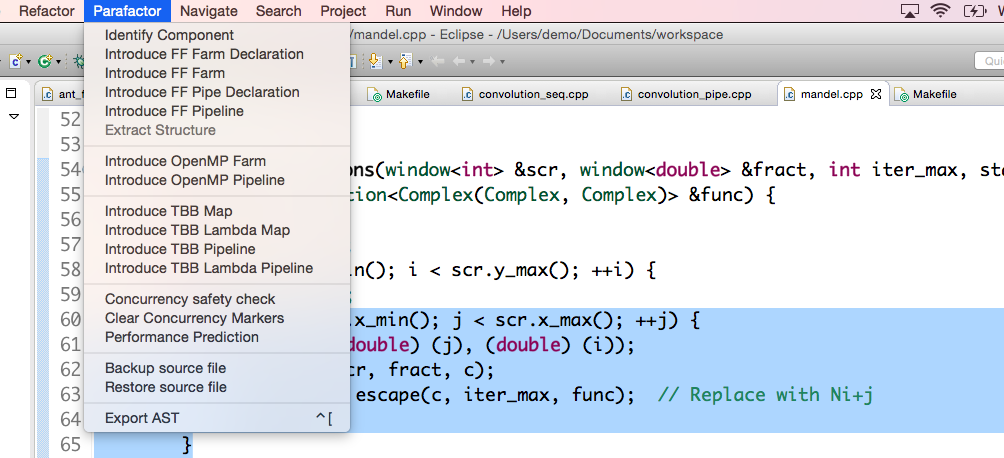
\includegraphics[width=0.95\linewidth]{figures/parformance.png}
\caption{The ParaFormance Refactoring Tool in Eclipse}
\label{eclipse}
\end{center}
\end{figure*}

\begin{figure*}
\begin{center}
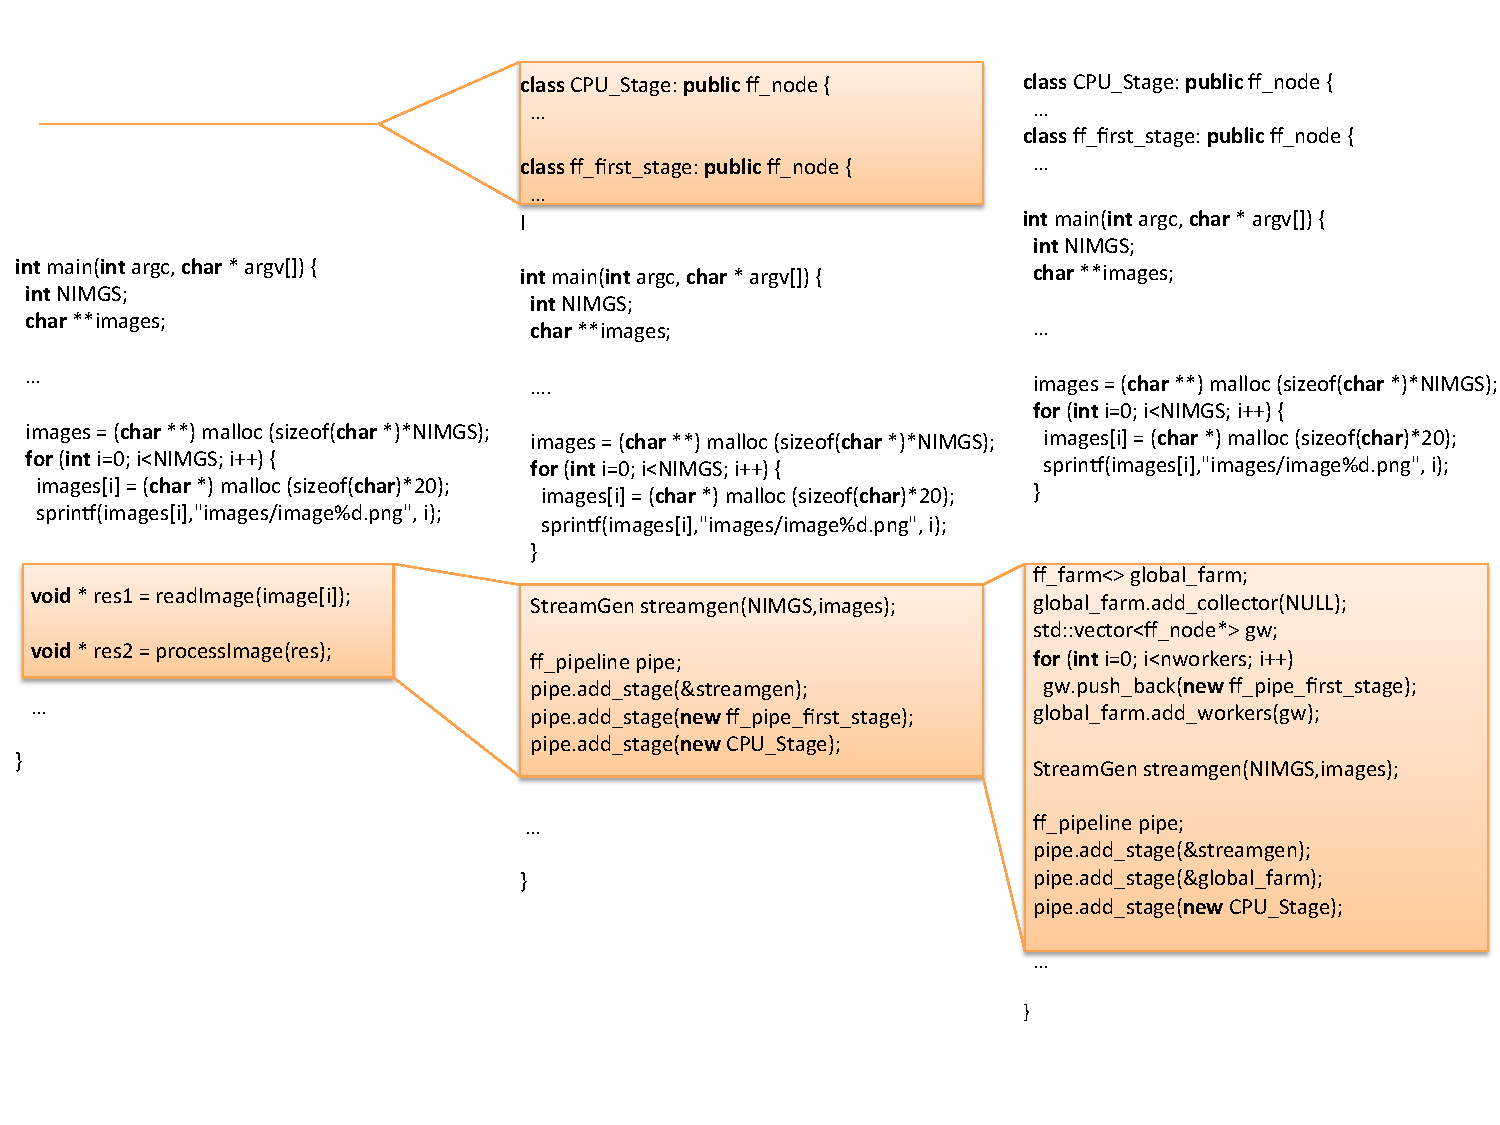
\includegraphics[width=0.99\linewidth]{figures/refactoring.pdf}
%\begin{minipage}{0.33\linewidth}
%\begin{scriptsize}
%\begin{lstlisting}[language=C++, caption=Sequential Version]
%struct Image 
%
%Image* georef(Image* image) {
%  ...
%
%Image* denoise(Image* image) {
%  ...
%
%int main(int argc, char* argv[]) {
%  ...
%  // the following part of code is 
%  // highlighted by the programmer
%  // in the refactoring tool
%  for(int i=0; i < N; i++) {
%     result1 = georef(inpt[i]); 
%     results[i] = denoise(result1);
%  }
%  // do something using the results 
%  // array
%}
%\end{lstlisting}
%\end{scriptsize}
%\end{minipage}%
%%\hfill\vrule\hfill
%\begin{minipage}{0.33\linewidth}
%\begin{scriptsize}
%\begin{lstlisting}[language=c++, caption=Introduce Pipeline]
%struct Image 
%
%Image* georef(Image* image) {
%  ...
%
%Image* denoise(Image* image) {
%  ...
%
%int main(int argc, char* argv[]) {
%  ...
% ff_pipeline pipe;
% StreamGen<Image> streamgen(NIMGS, 
%                            images);
% GenNode<Image> stage1(georef);
% GenNode<Image> stage2(denoise, 
%                       results);
% pipe.addStage(&streamgen);
% pipe.addStage(&stage1);
% pipe.addStage(&stage2);
% results = pipe.run_and_wait_end();
% 
% // do something using the results 
% // array
% 
%}
%\end{lstlisting}
%\end{scriptsize}
%\end{minipage}%
%\begin{minipage}{0.33\linewidth}
%\begin{scriptsize}
%\begin{lstlisting}[language=c++, caption=Introduce Farm]
%struct Image 
%
%Image* georef(Image* image) {
%  ...
%
%Image* denoise(Image* image) {
%  ...
%
%int main(int argc, char* argv[]) {
%  ...
% ff_pipeline pipe;
% StreamGen<Image> streamgen(NIMGS, 
%                            images);
% GenNode<Image> stage1(georef);
% GenNode<Image> stage2(denoise, 
%                       results);
% pipe.addStage(&streamgen);
% 
% ff_farm<> geoFarm;
%    std::vector<ff_node*> v;
%    for(int i=0;i<NW;++i) v.push_back(
%                 new GeoRef);
%    geoFarm.add_workers(v)
%
%    geoFarm.add_collector(NULL); 
% 
% pipe.addStage(&stage1);
% pipe.addStage(&stage2);
% results = pipe.run_and_wait_end();
% 
% // do something using the results 
% // array
%}
%\end{lstlisting}
%\end{scriptsize}
%\end{minipage}
\caption{The evolution of a skeleton program using refactoring: introduce a pipeline skeleton and then introduce a farm skeleton for a convolution algorithm.}
\label{refacex}
\end{center}
\end{figure*}

\subsection{FastFlow}
\noindent
FastFlow~\cite{AldinucciDKMT11} is a skeleton-based parallel programming framework
for multi-core platforms, implemented in C++.
% . FastFlow facilitates the development
% of shared-memory parallel applications by providing
% abstraction layers, programming constructs, and composable
% algorithmic skeletons~\cite{AldinucciDKMT11}.
FastFlow's streaming patterns are coordinating mechanisms
that control the flow of work between multiple concurrent
threads. This allows programmers to focus on
application-specific computational components by
abstracting over complex coordination and communication
layers. 
FastFlow supports both CPUs and GPUs as part of a heteogeneous parallel system~\cite{mpdp}.
% In~\cite{mpdp}, a heterogeneous skeletal framework was added to FastFlow which allows the programmer
% to incorporate the GPU code. 
% It should arguably be particularly useful in the
% context of heterogeneous multi-core CPU and GPU platforms.
% In~\cite{mpdp}, a heterogeneous skeletal framework was added to FastFlow which allows the programmer
% to incorporate the GPU code. 
% However the number of CPU/GPU workers allocated to each component remains a choice which has to be configured manually by 
% the programmer.

% VJ : eh?
% In~\cite{collinsoptimization} an empirical exploration of the optimisation space under the FastFlow framework was conducted. It was demonstrated 
% that a 70\% improvement for a particular FastFlow application was achieved by tuning the number of component instances and the connected 
% queue size of each component. This further motivates the need for auto-tuning.
\section{Monte Carlo Tree Search Model for Deriving Static Mappings}

\noindent
In this section, we describe a model that we use to derive, for a
given skeletal configuration, the best static mapping of its components to
the available hardware. A static mapping in our case corresponds to a
particular choice of values for the parameters of skeletons, i.e.\ the number of workers in
each farm, the type (CPU or GPU) of each worker in each farm and each stage of each pipeline. We
consider the best static mapping to be the one that
yields the best runtime for that particular skeletal
configuration.

%We consider a program factorised as a combination of parallel patterns. The factorisation gives rise to a process graph, the leaves of which represent particular units of computation, called functions, which will be allocated, in parallel, to a set of available processors. Processors can be of C (CPU) or G (GPU) type. Decisions must be made on how much computational resource and of which type (C or G) will be allocated to the parallel computation of each function. The Static Mapping Problem is to determine a fixed allocation of processing resource to functions to maximise the throughput of the parallel program.

%The process tree along with a policy defines a process graph which shows the sequence of processing starting from input running through a set of patterns. An input packet is passed to the first pattern. It passes through a series of structural boxes ending at a leaf which is the function for which it is the input. That function is executed on a processor selected by the policy. The outputs are then passed through the structure to the next function leaf and so on. This happens in parallel so that many sequences of processing are being executed in parallel.


%Our aim is to make available, in design time, a means of identifying an optimal static mapping with regard to throughput. Given the above assumptions, any parallel program may be characterised by its pattern tree and the set of distributions of function timings. For a fixed tree depth, it is possible to generate all possible abstract factorisations raising the possibility of similarity matching between parallel programs by structure and function profiles. Thus learning about optimal static mappings can potentially be transferred from stored calculations to new programs at the design stage.  Optimisation can be regarded as a search through possible static mappings with the aim of maximising throughput. 

Our model accepts as an input a skeletal configuration and the
the timings for its sequential components (both for CPU and
GPU versions, if the GPU version of a component is available). As an
output, it produces the best static mapping (according to a specific
evaluation function, $Q$) and the estimated runtime of the skeletal
configuration with that static mapping. Since considering all possible static mappings for a given
skeletal configuration may be computationally intractable, our model
uses the Monte Carlo Tree Search (MCTS) approach for generating and
evaluating large game trees in Game theory. In our case, in the
generated tree,  the inner nodes correspond to the partial mappings (with some of the
skeleton parameters chosen) and the leaves of the tree (with all parents to the root) corresponds to
the complete mappings (with all parameters of all skeletons
chosen). The children of a node, $v$, represent different possible
assignments of a yet unassigned skeleton parameter of incomplete
static mapping, $v$.

The MTCS approach starts from a tree that consists only of a
single 
root node (i.e.\ a static mapping where no
parameters for any skeleton are chosen). It proceeds by repeating the following three steps: 
\begin{enumerate}
\item \emph{Expansion step} -- A node that corresponds to some
  partial static mapping is selected, and one of its children is
  added to the tree. This corresponds to assigning value for one
  parameter of one skeleton in our skeletal configuration;
\item \emph{Selection step} -- Starting from the newly added node, a
  complete static mapping is generated by randomly choosing the
  remaining skeleton parameters. Once this static mapping is
  generated, its runtime is estimated using simulations, and the
  evaluation function, $Q$, is applied to that mapping and the runtime,
  giving a valuation, $v$;
\item \emph{Propagation step} -- The valuation, $v$, is propagated back
  to the node added in step $1$, and that node is assigned a valuation
  $v$. 
\end{enumerate}

The algorithm terminates, when after $K$ iterations, no new solutions have been generated.
At this point, from the root node to the leaf,
the children with both the highest 
visit count and the highest valuation, $v$, will be selected. This branch corresponds to the static mapping that is returned by the model.


% VJ : Something is obviously missing here

% A challenge is then to
%efficiently gain sufficient information from the simulation 
% to discriminate between mappings with a level of confidence.
% In order to customise the MCTS for our static mapping problem,
% we model the allocation as a sequence of decisions that determines the quantity of 
% the available remaining resource that should be allocated to a particular component. At each decision point, some resources will be allocated, 
% limiting the resources available to, as yet, unallocated components. We reach a leaf of the tree precisely when all components have been allocated 
% an amount and type of resource (which in pathological cases may be zero). At this point the mapping can be evaluated by simulation. We will apply 
% MCTS to search for an optimal path through this decision tree. The order of decisions is determined by the queue bottleneck. So the first 
% children of the tree will be the queue with the least throughput, the second level will be the second least throughput queue, and so on. This 
% creates a decision tree that is perfectly suitable for breadth-first search algorithms.

%Therefore, a given static mapping allows a simulation of the computation as random-walks where, at each step, a decision is made to allocate a 
%particular package of processing to a particular processor. The walk is biased by the parameters of the static mapping. At the end of the walk, 
%an evaluation function is calculated to measure the performance distributions on the assigned processors.

%The evaluation function is based on the throughput of the system which we denote by $T$.
%There are two balancing factors relating to the number 
%of resources allocated to the components of the system.
%$SD_U$ is the standard deviation of  the utilisation of all components in the system:

The evaluation function that we use to evaluate how good static
mappings are is based on the estimation of the runtime for that static
mapping that we obtain using simulations, and the utilisation of the
system. The function is

% VJ : What are queues, components? I don't get this
$$Q(v) = S(v) - (\delta_U(v) + \delta_Q(v)),$$
where $S(v)$ is the estimated throughput of the whole system,
$\delta_U(v)$ is the standard deviation of the utilisation of
components and $\delta_Q(v)$ is the standard deviation of
the utilisation of the connecting queues between the components in the skeleton. Using this function, $Q(v)$, rather than using
just the throughput, $S(v)$, as an evaluation function, discourages our
model for allocating more resources to the skeleton configuration, if
it only results in marginally improved runtime, which may be important
in settings where resources are paid for (e.g.\ clouds).

%$SD_U = \sqrt{\frac{\Sigma_{N}(U_{w_i}-U{w_{m}})^2}{N}}$

%Here, $N$ is total number of component sin the system, $U_{w_i}$ is the utilisation of the component, and $w_i$ and $U_{w_{m}}$ are the average utilisation values of all components in the system. 
%Adjusting the reward for this factor discourages the allocation of additional resources to components of queues  which are no longer bottlenecks.

%$SD_Q$ is the standard deviation of all queues in the system, defined:

%$SD_Q = \sqrt{\frac{\Sigma_{L}(T_{Q_i}-T_{Q_{m}})^2}{L}}$

% Here, $L$ is the total number of queues in the system, $T_{Q_i}$ is the throughput of the $Q_i$, and $T_{Q_{m}}$ is the average
% value of the throughput of all queues in the system. 
% Adjusting the reward for this factor discourages the allocation of additional resources to the components of a queue when they are no longer bottlenecks for that queue.%this may need further explanation

% Adding these two factors allows the algorithm to find the optimum 
% number of resources for the system, especially when the resources are, for example, on ``the cloud" where resources are typically expensive. Adding these two 
% penalty function can reduce the resource cost.

% Considering all these factors, the evaluation function $Q(v)$ for each selected path $v$ is defined:


% $Q(v) = T - (SD_{U} + SD_{Q})$ 
 
\section{Refactoring}
%[01/02/2013 15:57:38] Vladimir Janjic: skeleton rewrite rules are fine
%[01/02/2013 15:57:46] Vladimir Janjic: but they are abstract and not very usable, right?
%[01/02/2013 15:57:55] Vladimir Janjic: in order to apply them in a given language
%[01/02/2013 15:58:01] Vladimir Janjic: you still need to do all work yourself
%[01/02/2013 15:58:09] Vladimir Janjic: i.e. check that rules can be applied
%[01/02/2013 15:58:17] Vladimir Janjic: check that semantics is preserved
%[01/02/2013 15:58:22] Vladimir Janjic: and all that

\noindent
%% Intro/conclusion. KH
% We describe the refactorings here in terms of C++, but with a FastFlow
% skeleton approach, to demonstrate the principles of our methodology.  The
% refactorings could easily be demonstrated for other skeleton approaches
% and frameworks, and not are not limited to C++.  
Our refactoring
prototype is implemented in the ParaFormance (\url{http://www.paraformance.com}) tool, a refactoring tool-suite developed at the University of St Andrews that is integrated into Eclipse and Visual Studio, targetting both C and C++ via a variety of different backends (including Fastflow, Intel Thread Building Blocks (TBB), OpenMP and GrPPI).  
 The programmer is presented with a menu of possible refactorings to
apply.  The decision to apply a refactoring and identify a possible
skeleton to introduce is made by the programmer. Once a decision
has been made, any required transformation and mapping is performed automatically. In this way, we can rely on programmers making informed
decisions about which refactorings to apply, but do not rely on them % who may not have the
necessarily having expertise with parallelism or skeletons.  
In this paper, we make use of two new refactorings that introduce 

In this paper we make use of two refactorings previously described in~\cite{pdp2014}, where we introduced refactorings  such as
\emph{Introduce Farm} and \emph{Introduce Pipeline}. Below, we describe how these refactorings work over an Image Convolution example, shown in Figure~\ref{refacex}. %, which we discuss in more detail here.

\begin{itemize}
\item \textbf{Introduce Pipeline}.
% Here we define the \emph{Introduce Pipeline Refactoring}. 
For this refactoring, the programmer must select a \texttt{for} loop, e.g.,
the \texttt{for} loop that is shown in the first column of Figure \ref{refacex}.
The second column in the figure shows the effect after refactoring. % , which is a an \emph{automatic} transformation. 
% In the second column of the figure, 
Here, the original \texttt{for} loop has been re-written into a
\texttt{StreamGen} stage. This is a C++ class instance that models the
streaming input behaviour to the pipeline.  The refactoring is not
limited to only C style arrays, however, as C++ STL data structures may
also be considered, such as \texttt{std:vector< >} objects.  In the
second column, an instance of a FastFlow \emph{Pipe}line skeleton has
been introduced, named \texttt{pipe}.  The first stage, a function,
\texttt{ff\_pipe\_first\_stage}, is added as a pipeline stage; the second
stage, \texttt{CPU\_Stage}, is added as the final stage.  Finally, the
pipeline waits for the result of the computation, using a \texttt{run()}
method call.  The dependency between the output of
\texttt{ff\_pipe\_first\_stage} and the input of \texttt{CPU\_Stage} is
detected automatically. % by the refactoring.

\item \textbf{Introduce Farm}.
% Here we introduce the \emph{Introduce Farm Refactoring}, as demonstrated 
%This is shown in the third column of Figure \ref{refacex}.
  Here the refactoring has two variants: farming a \emph{Pipe}line stage;
  or, alternatively, introducing a new \emph{Farm}.  Farming a pipeline
  stage is the simplest of the two variants.  The middle column of
  Figure~\ref{refacex} shows a stage of an already defined FastFlow
  \emph{Pipe}line skeleton that the programmer has highlighted.  The
  result of the refactoring is shown in the right column: the \emph{Pipe}
  skeleton has been modified to replace the selected stage---here, the
  function \texttt{ff\_pipe\_first\_stage}---with a FastFlow \emph{Farm},
  called \texttt{global\_farm}. All other stages in the \emph{Pipe}line
  are preserved. The refactoring requires that \texttt{nworkers} (the
  number of \emph{Farm} workers) to be either previously defined, or given as an
  explicit argument to the refactoring.
\end{itemize}
Each of the introduction refactorings has a corresponding inverse:  \emph{Farm Elimination} inverts \emph{Introduce Farm};
 \emph{Pipeline Elimination} inverts \emph{Introduce Pipeline}. This allows any
combination of rules to be inverted, or undone, as part of a 
parallel refactoring process.  The refactorings are also fully nest-able,
allowing, for example, a farm, such as $\Delta(f1 \circ f2)$ (a task farm
where the worker is a function composition of two components, \emph{f1}
and \emph{f2}), to be refactored into $\Delta(f1 \parallel f2)$.

%\subsection{Tuning Parallelism}
%\begin{itemize}
%\item \textbf{Skeleton Tree to Skeleton Tree}
%\item \textbf{Chunking}
%\item \textbf{GPU Variants}
%\end{itemize}

\section{Results} \label{sec:results}

In this section, we demonstrate our technique on a convolution algorithm, which we describe in Section~\ref{sec:convolution} showing 
a number of different potential configurations of the algorithm in Section~\ref{sec:configurations}. We then take the three most optimal configurations,
based on a pre-filtering stage by applying high-level abstract cost models (Section~\ref{sec:costmodels}) to eliminate weak candidates. The remaining configurations are then passed
through our MCTS model, which predicts optimal mappings for each configuration. The application is then refactored for each configuration and mapping, where
we show that the actual performance speedups of the different configurations match the mappings from the MCTS in Section~\ref{sec:performance}.

\subsection{The Convolution Algorithm} \label{sec:convolution}
\noindent
Image convolution is a technique widely used in image processing applications such as blurring, smoothing
or edge detection. 
The basic structure of our convolution algorithm is a two-stage function composition, $ r \circ p $, where
$r$ is a stage that reads in an image from a file, and $p$ is a stage that processes the image, by applying a filter to the image. This convolution process is typically applied to a stream of input images, where the output is also a stream of (filtered) images.
Computationally, the filtering stage requires a scalar product of the filter weights with the input pixels within a window surrounding
each of the output pixels:
\begin{multline}
\label{eqn:01}
output\_pixel(i,j)=\sum_{m}\sum_{n} input\_pixel(i-n,j-m)\times\\
filter\_weight(n,m){}
\end{multline}
% The Heterogeneous FastFlow framework has been presented in~\cite{mpdp}. 
In order to develop the convolution problem for a
heterogeneous system, using FastFlow, we created a subclass \texttt{ff\_node} to implement $r$ (which cannot be executed on a GPU).
To implement the second stage, $p$, to execute on a GPU, we created a subclass, \texttt{ff\_gpu\_solve} which is derived from
\texttt{ff\_oclNode}. % More Details implementation of the FastFlow convolution problem can be found in~\cite{mpdp}.

\subsection{Cost Models} \label{sec:costmodels}
\noindent
In this section we give a corresponding high-level cost model for each
skeleton in Section \ref{sec:skeletons}, derived after those presented in  \cite{DBLP:books/daglib/0098705,DBLP:conf/europar/CaromelL07}. 
These cost models capture the service time of our skeletons and
will be used to filter the enumerated skeleton configurations, eliminating
candidates that will obviously yield poor performance results.
In order to demonstrate the principles of our methodology, the cost models
that we consider here are intentionally high-level and simple, abstracting over
many language- and architecture-specific details. Their only purpose is to give us
an rough performance estimate for each configuration.
%% Do they? KH
% , resulting in cost models that are naturally yield a best-case performance prediction. 
If desired, more complex models could be used to yield more accurate
predictions for a specific architecture,
without changing the general methodology.

\noindent
Function \emph{Comp}osition ($\circ$) can be costed trivially:
\begin{equation}
T_{C_{\circ}}(L) = l * (\sum_{1}^{m}{T_{stage_{m}}})
\end{equation}
where $L$ represents the maximum size of the input list and  $m$ represents the number of stages.
%We assume that all input tasks are \emph{regular}, i.e. the cost of the computation is fixed and does not depend on the size of the input task.
A suitable average-case cost model for the parallel \emph{Pipe}line is ($\parallel$):
%\begin{equation}
 % T_{C_{pipeline}} (L) = Max(T_{Stage_{1}} (L), T_{Stage_{2}} (L), ... , T_{{Stage}_{n}} (L)) + T_{copy} % (T_{copy} * (n-1))
%%  T_{C_{map}}(N_{w}, L) = T_{distrib}(N_{w}, L) + \frac{T_{Fun}(L)}{N_w} +
%%T_{gather}(N_{w}, L)  \label{map:tc}
%\end{equation}

% $oneStage1 + $oneStage2 + ($ninputs - 2) * max($oneStage1,$oneStage2);

\begin{multline}
T_{C_{\parallel}}(L) = \\ ( \sum_{1}^{m}{T_{stage_{m}}}) + (L - m) * \left( max_{(i=1..m)} T_{stage_{i}})\right)
\end{multline}

\noindent
%where $L$ represents the length of the input (and output) list.
% where $n$ is the number of inputs.
This defines the cost of a steady-state pipeline in terms of the
initial cost of filling the pipeline, plus the maximum execution cost for
any of the stages of the pipeline multiplied by the number of inputs minus the number of stages 
(we have already accounted for $m$ stages in the initial stage of filling the pipeline).

%This defines the cost of a steady-state pipeline as the total time taken by the pipeline stages divided by the minimum of the number
%of workers or the number of tasks plus the number of stages in the pipeline.
%

%
%The  times for distributing and gathering results represent the serial fraction of our parallel
%algorithm. By Amdahl's law, speedup will thus be bounded by:
%\begin{equation}
%\begin{array}{lcl}
%S_{map}(L) & ~=~ &\frac{T_{Fun}(L)}{ \frac{T_{Fun}(L)}{N_{w}} + T_{distrib}(N_{w}, L) + T_{gather}(N_{w}, L)}\\[2ex]
%&&  \texttt{where} ~~N_{W} = npartititions (L)
%\end{array}
%\end{equation}
%
% Taking into account the map implementation in Erlang outlined above, 

%
For the \emph{Farm} skeleton ($\Delta$), 
assuming that each worker task has a similar granularity and that all
workers are fully occupied, the corresponding cost model is: % to the farm skeleton:
%$time = $tcomp * ceil ( $ninputs / min ($ncores, $nworkers) ) + ($tdist + $tgather) * min ($ncores, $ninputs);

\begin{multline}
T_{C_{\Delta}}(N_{p}, N_{w}, L) = \\ T_{worker} * \lceil \frac{L}{min(N_{p}, N_{w})} \rceil + (T_{dist} + T_{gather}) * min (p, L)
\end{multline}

\noindent
For our  FastFlow definition, more accurate definitions of $T_{dist}$ and $T_{gather}$ are:
\begin{multline}
T_{dist}(N_w,L) = N_w \cdot T_{spawn} + N_w \cdot (T_{setup} + T_{copy}(\frac{L}{N_{w}})) \\
T_{gather}(N_w,L) = N_w \cdot (T_{setup} + T_{copy}(\frac{L}{N_{w}})) 
\end{multline}

\noindent
Here, $N_{p}$ is the total number of cores (including GPU elements), $N_{w}$ is the number of workers, and $L$ is the size of the input list.
The cost of a farm is defined as the cost of the $worker$ function times the ceiling of the number of inputs divided by the minimum of the number of cores and the number of workers. This is added to the time to distribute and gather the results, multiplied by the minimum of the number of inputs or the number or workers.

%\begin{small}
%\begin{equation}
%  T_{C_{farn}}(N_{w}, L) =  \\ max \{ T_{emitter}(N_{p, N_{w}}, L) , \frac{T_{Fun}(L)}{Min(N_p, N_w)} ,
%T_{collector}(N_{w}, L) \}  \label{map:tc}
%\end{equation}
%\end{small}

\subsection{Configurations} \label{sec:configurations}
%\begin{small}
%\begin{tabular}{| r | l | l | l |}
%\hline
% & Configuration & CPU Time & GPU Time \tabularnewline
%\hline
%\hline
%1 & $ Seq(r) \circ Seq(p) $ & 136.00 & 5.60  \tabularnewline
%\hline
%2a & $Pipe(Seq(r), Seq(CPU(p)))$ & 125.60 \tabularnewline
%\hline
%2b & $Pipe(Seq(r), Seq(GPU(p)))$ & 3.88 \tabularnewline
%\hline
%3 & $Pipe(Farm(Seq(r)), Seq(p))$ & 132.00 \tabularnewline
%\hline
%4 & $Pipe(Seq(r), Farm(Seq(p)))$ \tabularnewline
%\hline
%5 & $Pipe(Farm(Seq(r)), Farm(Seq(p)))$\tabularnewline
%\hline
%6 & $Farm(Pipe(Seq(r),Seq(p)))$\tabularnewline
%\hline
%7 & $Farm(Comp(Seq(r), Seq(p))$\tabularnewline
%\hline
%8 & $Comp(Farm(Seq(r), Farm(Seq(p))))$\tabularnewline
%\hline
%9 & $Comp(Farm(Seq(r), Seq(p)))$ \tabularnewline
%\hline
%10 & $Comp(Seq(r), Farm(Seq(p)))$\tabularnewline
%\hline
%\end{tabular}
%\end{small}

\begin{figure}
\begin{center}
\begin{tabular}{| r | l | l | l |}
\hline
 & Configuration & CPU Time & GPU Time \tabularnewline
\hline
\hline
1 & $ r \circ p $ & 136.00 & 5.60  \tabularnewline
\hline
2 & $r \parallel p$ & 125.60 & 3.88 \tabularnewline
\hline
\textbf{3} & $ \mathbf{\Delta(r) \parallel p}$ & \textbf{132.00} & \textbf{1.60} \tabularnewline
\hline
4 & $ r \parallel \Delta(p)$ & 13.20 & 4.00 \tabularnewline
\hline
\textbf{5} & $\mathbf{\Delta(r) \parallel \Delta(p)}$ & \textbf{13.20} & \textbf{0.40}  \tabularnewline
\hline
\textbf{6} & $\mathbf{\Delta(r \parallel p)}$ & \textbf{13.60} & \textbf{0.56}  \tabularnewline
\hline
7 & $\Delta(r \circ p)$ & 13.60 & 5.60  \tabularnewline
\hline
8 & $\Delta(r) \circ \Delta(p)$ & 13.60 & 2.00  \tabularnewline
\hline
9 & $\Delta(r) \circ p$ & 132.40 & 2.00 \tabularnewline
\hline
10 & $r \circ \Delta(p)$ & 17.20 & 5.60 \tabularnewline
\hline
\end{tabular}
\caption{Cost predicted runtimes (in milliseconds) for both CPU and GPU versions of the possible configurations of convolutions (up to depth 2)}
\label{fig:configs}
\end{center}
\end{figure}
\noindent
The first step in our methodology is to take the initial
\emph{sequential} pattern tree that we have derived from the convolution
algorithm, and enumerate all possible configurations of the pattern tree
up to a given depth, $N$.  In order to demonstrate the principles of our
methodology, we choose to enumerate up to 2 nestings, resulting in 10
possible pattern-tree configurations, where each of the configurations
represents a refactoring candidate.  For our example, we consider
introducing a \emph{Farm} ($\Delta$) in both stages of the
\emph{Pipe}line ($\parallel$), this is justified by the fact that it is
plausible to read in multiple images from a database at the same time,
for example, when processing multiple medical images, or when reading
from multiple CCTV videos simultaneously~\cite{ediPhd}.  In
Figure~\ref{fig:configs}, we show the different possible pattern-tree
configurations for the convolution algorithm, up to a nesting depth of 2.
We also show the predicted runtimes of each configuration based on the
results of our high-level cost models for both a CPU and GPU. The times
shown are the best predictions for our 24-core testbed machine, based on the
following settings (obtained by profiling the application):
$L=20$, $r = 0.2ms $, $p_{CPU} = 6.6ms$, $r_{GPU} = 0.08ms$. Using these
profiling results, we can instantiate the cost models from the
previous section, using profiling, to give a minimal
$T_{gather}=0.001ms$ and $T_{dist}=0.001ms$.  The high-level cost models
give us an estimated minimal runtime for each configuration, which we can
use to filter out weak candidates. Based on the cost model predictions,
we isolate the top three configurations as candidates for our MCTS model.
These candidates are shown in bold in Figure~\ref{fig:configs}.

\begin{figure}
\begin{center}
\begin{tabular}{| r | l | l | l | l |}
\hline
 &  $ \Delta(r) \parallel \Delta(p) $ &  $\Delta(r) \parallel p$ & $\Delta(r \parallel p)$ \tabularnewline
\hline
\hline
GPU & 3 & 1 & 5  \tabularnewline
\hline
CPU & 6 & 4 & 5 \tabularnewline
\hline
\end{tabular}
\caption{MCTS predicted optimal mappings for three configurations showing number of workers for both CPU and GPU}
\label{fig:predicts}
\end{center}
\end{figure}

\subsection{Performance Results} \label{sec:performance}
\noindent
All measurements have been made on an 2x 2.4Ghz 12-core AMD Opteron 6176 CPUs coupled an NVidia Tesla C2050 with 448 GPU
cores running at 1.16GHz, running Centos Linux 
2.6.18-274.el5. and g++ 4.1.2, averaging over 10 runs with an image size of $4096*4096$ applied to a stream of images.

\begin{figure}
\begin{center}
\begin{tikzpicture}
\begin{axis}[
  mark size=0.6mm,
  cycle list={
    {blue,mark=star},
    {red,mark=diamond},
    {brown!60!black,mark=triangle},
    {blue,dashed,mark=star},
    {red,dashed,mark=diamond},
    {brown!60!black,dashed,mark=triangle},
  },
  legend style={
    font=\small,
    cells={anchor=west},
  },
  legend pos= north east,
  enlargelimits,
  xtick={1,4,8,12,16},
  ytick={1,5,10,15,20,25,30,35,40},
  %ymin=1,
  ymax=40,
  xlabel=No. CPU Workers,
  ylabel=Speedup,
  title=Speedups for $\Delta(r) \parallel p$
  ]
\addplot table[x index=0,y index=1] {results/version3.txt};
\addlegendentry{ $GPU = 1$}
%\addplot table[x index=0,y index=3] {Actual2.txt};
%\addlegendentry{Farm with Chunk 16}
%\addplot table[x index=0,y index=2] {Predicted2.txt};
%\addplot table[x index=0,y index=3] {Predicted2.txt};
%\addplot table[x index=0,y index=4] {Predicted2.txt};
\end{axis}
\end{tikzpicture}
\caption{Speedup graph for configuration 3, for 1 GPU worker}
\label{ver1}
\end{center}
\end{figure}
Figure~\ref{ver1} shows the actual speedup results for $ \Delta(r) \parallel p $ (version 3, from Figure~\ref{fig:configs}).
For this configuration, the second stage of the \emph{Pipe}, $p$, is a single worker, so only 1 GPU worker is considered.
The MCTS predicts for this configuration (from Figure~\ref{fig:predicts}) an optimal mapping allocating 4 CPU workers and 1 GPU worker. As Figure~\ref{ver1} shows, 
4 CPU workers and 1 GPU worker gives an actual speedup of 39.14, compared with a best performance speedup of 39.43, for 8 CPU workers and 1 GPU worker, this mapping prediction is within $1\%$ of the best speedup obtained for this configuration.
The difference between 4 CPU workers and 8 CPU workers is a minimal speedup of 0.29.
This is rejected as a candidate solution since the MCTS also takes into account hardware utilisation.
Using an additional 4 CPUs to gain such a small increase in speedup will usually not be worthwhile. 
% This may be the case if, for example, the application is ran on a cloud infrastructure, where buying more CPU nodes becomes expensive, or in situations where energy properties also need to be considered. 

\begin{figure}[t]
\begin{center}
\begin{tikzpicture}
\begin{axis}[
  mark size=0.6mm,
  cycle list={
    {blue,mark=star},
    {red,mark=diamond},
    {brown!60!black,mark=triangle},
    {green,mark=star},
    {red,dashed,mark=diamond},
    {brown!60!black,dashed,mark=triangle},
  },
  legend style={
    font=\small,
    cells={anchor=west},
  },
  legend pos= north east,
  enlargelimits,
  xtick={1,4,8,12,16},
  ytick={1,5,10,15,20,25,30,35,40,45},
  %ymin=1,
  ymax=45,
  xlabel=No. CPU Workers,
  ylabel=Speedup,
  title=Speedups for $\Delta(r) \parallel \Delta(p)$
  ]
\addplot table[x index=0,y index=1] {results/version51GPU.txt};
\addlegendentry{ $GPU = 1$}
\addplot table[x index=0,y index=1] {results/version53GPU.txt};
\addlegendentry{$GPU = 3 $}
\addplot table[x index=0,y index=1] {results/version55GPU.txt};
\addlegendentry{$GPU = 5 $}
\addplot table[x index=0,y index=1] {results/version57GPU.txt};
\addlegendentry{$GPU = 7 $}
%\addplot table[x index=0,y index=2] {Predicted2.txt};
%\addplot table[x index=0,y index=3] {Predicted2.txt};
%\addplot table[x index=0,y index=4] {Predicted2.txt};
\end{axis}
\end{tikzpicture}
\caption{Speedup figures for configuration 5 for 1,3,5, and 7 number of GPU workers} 
\label{ver2}
\end{center}
\end{figure}
In Figure~\ref{ver2} we show the speedups for $\Delta(r) \parallel \Delta(p)$ (configuration 5, as shown in Figure~\ref{fig:configs}).
The figure shows speedup figures for the configuration with a variety of GPU workers (here, 1,3,5 and 7 GPU workers), where
we decided to show the best speedups, where other runs with a different numbers of GPU workers (up to 16 GPU workers) showed much poorer speedup results and 
were deemed uninteresting.
For this configuration, the MCTS prediction (from Figure~\ref{fig:predicts}) shows optimal speedup for 6 CPU workers and 3 GPU workers, 
however Figure~\ref{ver2} shows, for 6 CPU and 3 GPU workers, a speedup of 39.12, where the best speedup is for 4 CPU and 3 GPU workers, with a speedup of 40.91.
This demonstrates that our MCTS prediction for this configuration is within $4\%$ of the best speedup obtained.
From Figure~\ref{ver2}, we can also see that from the remaining performance measurements, the best speedup for 1 GPU worker is 39.35 (for 5 CPU workers), 5 GPU workers is 40.08 (for 4 CPU workers) and 7 GPU workers is 28.39 (for 4 CPU workers).

\begin{figure}
\begin{center}
\begin{tikzpicture}
\begin{axis}[
  mark size=0.6mm,
  cycle list={
    {blue,mark=star},
    {red,mark=diamond},
    {brown!60!black,mark=triangle},
    {blue,dashed,mark=star},
    {red,dashed,mark=diamond},
    {brown!60!black,dashed,mark=triangle},
  },
  legend style={
    font=\small,
    cells={anchor=west},
  },
  legend pos= north east,
  enlargelimits,
  xtick={1,4,8,12,16},
  ytick={1,2,3,4,5,6,7,8,9,10},
  %ymin=1,
  ymax=10,
  xlabel=No. CPU Workers,
  ylabel=Speedup,
  title=Speedups for $\Delta(r \parallel p)$
  ]
\addplot table[x index=0,y index=1] {results/version107GPU.txt};
\addlegendentry{ $GPU = No.\ CPU\ Workers$}
%\addplot table[x index=0,y index=3] {Actual2.txt};
%\addlegendentry{Farm with Chunk 16}
%\addplot table[x index=0,y index=2] {Predicted2.txt};
%\addplot table[x index=0,y index=3] {Predicted2.txt};
%\addplot table[x index=0,y index=4] {Predicted2.txt};
\end{axis}
\end{tikzpicture}
\caption{Speedup figures for configuration 6, where the number GPU workers = number CPU workers}
\label{ver3}
\end{center}
\end{figure}

Figure~\ref{ver3} shows the speedups for $ \Delta(r \parallel p)$ (configuration 6, as shown in Figure~\ref{fig:configs}). Here
we show for each speedup of $n$ CPU workers and also $n$ GPU workers. Other results showed much poorer speedups and
we therefore have not shown them here. % deemed them uninteresting to show.
As Figure~\ref{ver3} demonstrates, the best speedup obtained for this configuration is 7.45 for 5 CPU and 5 GPU workers, which confirms the
prediction given by our MCTS model (Figure~\ref{fig:predicts}).

It is noted that the speedup figures here do not always show smooth performance improvements by increasing the number of workers, and there are points where we even get poor performance (such as in Figure~\ref{ver2} for 9 CPU workers and 5 GPU workers).
One possible reason for this could be that we have a combination of nodes where each node
gives a different service time: increasing the number of workers only to the \emph{bottleneck} stages
increases global throughput, and therefore performance.
Once the bottleneck has been removed, adding any extra workers to a 
non-bottleneck stage in FastFlow doesn't always seem to improve the performance, since there is extra overhead in the system from creating the extra thread. FastFlow is designed for fine-grained parallelism, with an assumption
that most of the stages are CPU bound. 
This gives rise to a problem when addressing computations that are assigned to the GPU, where increasing the number of GPU workers can
actually harm the performance rather than improve it, especially when the allocation of tasks to the GPU no longer fits into the GPU model.
Our MCTS model compensates for this, by finding an optimal result by considering the utilisation of stages as a penalty factor in the system.
In addition, the cost model predictions for the configurations, from Figure~\ref{fig:configs}, predicted that the second most optimal configuration is $\Delta(r  \parallel p)$. However, looking at the actual performance measurements, $ \Delta(r) \parallel p $ performs better, with an increased speedup of $31.98$ over the $\Delta(r \parallel p)$ configuration. This shows that using high-level cost models alone is not enough to predict optimal parallelisations.

\section{Related Work}
\subsection{Static Mapping}

\noindent
The static mapping problem is by no means a new challenge and there is an extensive body
of work on mapping task, data and pipeline parallelism to
parallel architectures providing static
partitioning~\cite{kwok1999static,saraswat2007x10,subhlok1993exploiting}, using runtime scheduling~\cite{distributed1984dynamic}, heuristic-based
mappings~\cite{gordon2006exploiting}, analytical models~\cite{culler1996logp,navarro2009analytical}, 
or ILP solvers~\cite{kudlur2008orchestrating}. Each of these can improve the performance of the system.
There are some heuristic based approaches which automate the process of mapping to multi-core architectures for specific frameworks, such as 
the learning approach used for partitioning streaming in the StreamIt framework~\cite{wang2010partitioning} or the runtime adaptation 
approach used in FlexStream~\cite{hormati2009flextream} framework. Also, a recent series of research aims at 
optimising the use of resources on multi-core embedded platforms linking both design-time optimisation and simulation with run-time optimisation using lightweight 
heuristics~\cite{ykman2010exploration,ykman2007design,ykman2011linking}. In~\cite{avasare2010practical}, the use of 
platform simulators has been considered 
to identify Pareto-optimal design configurations of parallel applications 
(incorporating code versions, resource mappings, constraints and costs).
Despite the amount of work done in the homogeneous environment, to our best knowledge there is little work done for mapping to 
heterogeneous (CPU/GPU) architectures. Most of the work on GPUs is primarily focused on application performance 
tuning~\cite{agrawal2005optimizing} rather than orchestration.
In~\cite{udupa2009software} a method is provided to orchestrate the execution of heterogeneous StreamIt program presented 
on a multi core platform equipped with an accelerator. They use integer
linear programming (ILP) formulations to perform partitioning over the combination of CPU/GPU.
Formulating ILP models, however, requires expert
knowledge of the underlying architecture. Finding a
solution under certain constraints for the ILP formula can
be time-consuming as well.
Our aim in this paper is automatic orchestration of CPU/GPU component for FastFlow applications by using MCTS which usually requires less knowledge
about the system. Therefore, minimum information is needed to run the result on the system. Moreover, applying it in a static manner has a much lower overhead
for deployment.

\subsection{Monte Carlo Tree Search}

\noindent
Monte Carlo Tree Search have classically been applied to challenging game playing, for example the GO and Bandit 
problem~\cite{coulom2007efficient,kocsis2006bandit,chaslot2006monte,gelly2006exploration}.
Recently MCTS has been applied to planning and scheduling problems. In~\cite{chaslot2006montep} a MonteCarlo search algorithm has been applied 
to produce management problems which can be defined as single-agents selecting a sequence of actions with side effects, 
leading to high quantities of one or more goal products. The result shows that they achieve a successful solution in less time than 
already existing learning method. In~\cite{nakhost2009monte} a Monte Carlo Random Walk (MRW) planning algorithm is used in 
deterministic classical planning achieving results comparable with the other state of the art algorithms. 
In~\cite{couetoux2011continuous} an extended version of UCT approach has been successfully applied in continuous stochastic problems with continuous action space. 
In this paper we establish the applicability of MCTS to the seamless orchestration of heterogeneous components over a hybrid(CPU, GPU) platform.
Although we work on the FastFlow framework, the techniques introduced here can easily be applied to a different framework by changing the evaluation method.
This makes the algorithm framework independent. 

\subsection{Refactoring}
\noindent
%Program transformation has a long history, with early work in the field being described by Partsch and Steinbruggen in 1983 \cite{partsch83}, and
%% For an extensive survey of refactoring tools and techniques, 
%Mens and Tourw\'{e} producing an extensive survey of refactoring tools and techniques in 2004 %  detailing the most common refactoring tools and practices 
%\cite{mens_refactoring}. 
%The first refactoring tool system was the \emph{fold/unfold} system of Burstall and Darlington \cite{darlington77} which was intended to transform recursively defined functions. 
%There
%are six basic transformation rules that the system is based on: unfolding; folding; instantiation; abstraction; definition and laws. The advantage of using this
%methodology is that it deployed a number of simple, and yet effective, structural program
%transformations that aimed to develop more efficient definitions; the disadvantage is that the use of the fold rule sometimes resulted in non-terminating definitions.
%
%The Haskell Refactorer, HaRe, is a semi-automated refactoring tool for sequential Haskell programs, developed at the University of Kent by Thompson, Li and Brown \cite{HaRe}.
%HaRe works over the full Haskell 98 standard, and contains a large catalog of refactorings that concentrate on small structural changes in sequential Haskell programs, such as \emph{renaming}, \emph{lambda lifting} and type-based refactorings. 
%Wrangler \cite{wrangler}, also developed at the University of Kent by Thompson and Li, is similar to HaRe, but works over sequential Erlang instead.
%Unlike our requirements for the \ParaPhrase{} project, Wrangler does not deal with parallel refactorings in any way.
% The University of Kent and E\"otv\"os Lor\'and University are now in the process
% of building refactoring tools for Erlang programs \cite{wrangler}. However, different techniques have been used to represent and manipulate the program under refactoring. The Kent approach uses the Annotated Abstract Syntax Tree (AAST)
% as the internal representation of an Erlang program, and program analyses and
% transformations manipulate the AAST directly.  
% %Wrangler also contains a large database of refactorings for Erlang programs and also includes a Domain Specific Language for expressing transformations (together with their conditions) \cite{wranglerdsl2} and also a further language for composing refactorings \cite{wranglerdsl}. 
% The E\"otv\"os L\"or\'and university
% approach uses the Erlang-based database Mnesia \cite{semantic09kept} to store both syntactic
% and semantic information of the Erlang program under refactoring; therefore,
% program analyses and transformations are carried out by manipulating the information stored in the database. 
There has so far been only a limited amount of work on refactoring for parallelism~\cite{fmcoover}. 
Hammond \emph{et. al} \cite{HammKBertJL2003:PPL} used Template
Haskell \cite{Sheard:2002} with explicit cost models to derive automatic farm skeletons for Eden
\cite{Breitinger96eden}. Unlike the approach presented
here, Template-Haskell is compile-time, meaning that the programmer
cannot continue to develop and maintain his/her program after the
skeleton derivation has taken place. Other work on parallel refactoring
has mostly considered loop parallelisation in Fortran \cite{reentrancy} and
Java \cite{dig}. However, these approaches are limited to concrete
structural changes (such as loop unrolling) rather than applying
high-level pattern-based rewrites as we have described here. 
%We have recently extended HaRe, the Haskell refactorer \cite{HaRe},
%to deal with a limited number of parallel refactorings \cite{paraform}.  
%This work allows Haskell programmers to introduce
%data and task parallelism using small structural refactoring steps.
However, it does not use pattern-based rewriting or MCTS based direction, as discussed in this
paper. 
%Recent work by Larsen et al.~\cite{larson}, describe an interactive refactoring approach 
%that takes the reports generated by optimising compilers and presents them to the user, so that hand-tuned optimisations can then take place to fix optimisation weaknesses. However, this approach relies on compilers with automatic parallelisation techniques, provided by pre-processing pragmas, rather than an approach exploits a disciplined methodological approach using skeletons and MCTS simulations.
%% complementary paper \emph{The ParaPhrase Project: Parallel Patterns for Adaptive Heterogenous Multicore Systems} by Hammond \emph{et al.}
%\subsection{Skeletons}
%Since the 1990s, the skeletons research community has been actively
%working on high-level languages and methods for parallel programming
%\cite{cole-th,cole:manifesto:02,BotKu96,DGTJ95,P3L,HMK98}.
A rich set of skeleton rewriting rules have been studied and proposed in \cite{FAN:PPA:01,pdcs:nf:99,Gorlatch:99,SkillicornC95}.
When using skeleton rewriting transformations a set of functionally equivalent programs 
exploiting different kinds of parallelism is obtained. Cost models and evaluation
methodologies have also been proposed that can be used to determine the best of a set of 
equivalent parallel programs \cite{aldinuc:stream-data:98,SkillicornC95}. 
The methodology presented in this paper extends and builds on this
and similar work by providing refactoring tool-support
supplemented by a programming methodology that
aims to make structured parallelism more accessible to a wider audience.

\section{Conclusions and Future Work}
\noindent
This paper has described a new technique that employs new
refactoring and static mapping technology. Refactoring allows programmers
to refactor their programs, introducing and tuning parallelism, where the choice of the refactoring and hardware mapping is derived automatically.
We have described a number of novel refactorings implemented in Eclipse, for C++ and FastFlow, and also described
an MCTS algorithm capable of delivering accurate mapping predictions for a heterogenous machine (within $5\%$ of the best speedup obtained).
Our convolution benchmark has shown that even for an algorithm with relatively little structure, there would be many different
\emph{manual} refactoring choices to choose from. Instead, our approach 
provides accurate mapping information, and refactoring predictions, outperforming a standard set of cost models, allowing the programmer to concentrate on the
the correctness of the application, rather than the parallelisation. 

Although our technique is described in terms of C++ using FastFlow, the approach taken here is,
in fact, completely generic. The refactorings and skeleton could easily be carried over to different languages and frameworks, such 
as Cilk, OpenMP, etc. In particular, the MCTS algorithm is designed to be used with any skeleton framework, 
being fully parameterised over the overheads in the implementation. Our intention is that we will, in time, develop
a generic refactoring and mapping methodology capable of using a common set of refactoring rules and skeletons  

In the near future, we expect to extend our technique to cover a wide range of parallel skeletons
including parallel workpools, divide-and-conquer, map-reduce, bulk synchronous parallelism, and other domain-specific
parallel patterns, such as parallel Orbit enumerations.
In addition, we intend to demonstrate the use of our methodology on a further set of benchmarks, showing greater skeleton nesting and potential heterogeneity. We also intend to implement the dynamic remapping of the FastFlow program as an extension over the generated result of the static mapping approach.
A remaining issue for further investigation is the applicability of this approach over a distributed heterogeneous architecture, where the cost of transferring both components and
data over a network is accounted for in the simulation, as it affects the system performance and utilisation of components. 


 % use section* for acknowledgement
% \section*{Acknowledgment}
 %\noindent
 %This work has been supported by the European Union grants
 %ST-2010-248828 ``ADVANCE: Asynchronous and Dynamic Virtualisation through performance ANalysis to support Concurrency Engineering'', and IST-2011-288570 ``ParaPhrase: Parallel Patterns for Adaptive Heterogeneous Multicore Systems'',
 %ad by the UK's Engineering and Physical Sciences Research Council
 %grant EP/G055181/1 ``HPC-GAP: High Performance Computational Algebra."

% trigger a \newpage just before the given reference
% number - used to balance the columns on the last page
% adjust value as needed - may need to be readjusted if
% the document is modified later
%\IEEEtriggeratref{8}
% The "triggered" command can be changed if desired:
%\IEEEtriggercmd{\enlargethispage{-5in}}

% references section

% can use a bibliography generated by BibTeX as a .bbl file
% BibTeX documentation can be easily obtained at:
% http://www.ctan.org/tex-archive/biblio/bibtex/contrib/doc/
% The IEEEtran BibTeX style support page is at:
% http://www.michaelshell.org/tex/ieeetran/bibtex/
%\bibliographystyle{IEEEtran}
% argument is your BibTeX string definitions and bibliography database(s)
%\bibliography{IEEEabrv,../bib/paper}
%
% <OR> manually copy in the resultant .bbl file
% set second argument of \begin to the number of references
% (used to reserve space for the reference number labels box)
%\bibliographystyle{abbrv}
%\bibliography{paraphrase,paraphrase-pubs,skeletons,tfp2011,gpu-programming,ref}

\begin{thebibliography}{10}

\bibitem{chaslot2006montep}
G.~Chaslot, S.~De~Jong, J.-T. Saito, and J.~Uiterwijk, Monte-carlo Tree
 ÊSearch in Production Management Problems, in \emph{Proceedings of the 18th
 ÊBeNeLux Conference on Artificial Intelligence}, 2006, pp. 91--98.

\bibitem{distributed1984dynamic}
K~Ramamritham.
\newblock Dynamic Task Scheduling in Hard Real-time Distributed Systems.
\newblock in {J. of Software, IEEE 1(3), pages 65--75}.
\newblock 1984.

\bibitem{agrawal2005optimizing}
S.~Agrawal, W.~Thies, and S.~Amarasinghe.
\newblock Optimizing Stream Programs Using Linear State Space Analysis.
\newblock In {\em Proceedings of the 2005 international conference on
  Compilers, architectures and synthesis for embedded systems}, pages 126--136.
  ACM, 2005.

\bibitem{aldinuc:stream-data:98}
M.~Aldinucci, M.~Coppola, and M.~Danelutto.
\newblock Rewriting {S}keleton {P}rograms: {H}ow to {E}valuate the
  {D}ata-{P}arallel {S}tream-{P}arallel {T}radeoff.
\newblock In S.~Gorlatch, editor, {\em Proc of CMPP: Intl. Workshop on
  Constructive Methods for Parallel Programming}, pages 44--58. Fakult{\"a}t
  f{\"u}r mathematik und informatik, Uni. Passau, Germany, May 1998.

\bibitem{pdcs:nf:99}
M.~Aldinucci and M.~Danelutto.
\newblock {Stream Parallel Skeleton Optimization}.
\newblock In {\em Proc. of PDCS: Intl. Conference on Parallel and Distributed
  Computing and Systems}, pages 955--962, Cambridge, Massachusetts, USA, Nov.
  1999. IASTED, ACTA press.

\bibitem{AldinucciDKMT11}
M.~Aldinucci, M.~Danelutto, P.~Kilpatrick, M.~Meneghin, and M.~Torquati.
\newblock {Accelerating Code on Multi-cores with FastFlow}.
\newblock In {\em Euro-Par}, pages 170--181, 2011.

\bibitem{FAN:PPA:01}
M.~Aldinucci, S.~Gorlatch, C.~Lengauer, and S.~Pelagatti.
\newblock Towards {P}arallel {P}rogramming by {T}ransformation: {T}he {FAN}
  {S}keleton {F}ramework.
\newblock {\em Parallel Algorithms and Applications}, 16(2--3):87--121, Mar.
  2001.

\bibitem{avasare2010practical}
P.~Avasare, G.~Vanmeerbeeck, C.~Kavka, and G.~Mariani.
\newblock Practical Approach for Design Space Explorations Using Simulators at
  Multiple Abstraction Levels.
\newblock In {\em Proc. Design Automation Conf. User Track, Anaheim, CA}, 2010.

\bibitem{DBLP:conf/europar/CaromelL07}
D.~Caromel and M.~Leyton.
\newblock Fine Tuning Algorithmic Skeletons.
\newblock In A.-M. Kermarrec, L.~Boug{\'e}, and T.~Priol, editors, {\em
  Euro-Par}, volume 4641 of {\em Lecture Notes in Computer Science}, pages
  72--81. Springer, 2007.

\bibitem{chaslot2010monte}
G.~Chaslot.
\newblock {\em Monte-carlo Tree Search}.
\newblock PhD thesis, Maastricht Univ, 2010.

\bibitem{chaslot2006monte}
G.~Chaslot, S.~De~Jong, J.~Saito, and J.~Uiterwijk.
\newblock Monte-carlo Tree Search in Production Management Problems.
\newblock In {\em Proceedings of the 18th BeNeLux Conference on Artificial
  Intelligence}, pages 91--98, 2006.

\bibitem{collinsoptimization}
A.~Collins, C.~Fensch, and H.~Leather.
\newblock Optimization Space Exploration of the Fastflow Parallel Skeleton
  framework.

\bibitem{couetoux2011continuous}
A.~Cou{\"e}toux, J.~Hoock, N.~Sokolovska, O.~Teytaud, and N.~Bonnard.
\newblock Continuous Upper Confidence Trees.
\newblock {\em Learning and Intelligent Optimization}, pages 433--445, 2011.

\bibitem{coulom2007efficient}
R.~Coulom.
\newblock Efficient Selectivity and Backup Operators in Monte-carlo Tree
  Search.
\newblock {\em Computers and Games}, pages 72--83, 2007.

\bibitem{culler1996logp}
D.~E. Culler, R.~M. Karp, D.~Patterson, A.~Sahay, E.~E. Santos, K.~E. Schauser,
  R.~Subramonian, and T.~von Eicken.
\newblock Logp: A Practical Model of Parallel Computation.
\newblock {\em Communications of the ACM}, 39(11):78--85, 1996.

\bibitem{dig}
D.~Dig.
\newblock A {R}efactoring {A}pproach to {P}arallelism.
\newblock {\em IEEE Softw.}, 28:17--22, January 2011.

\bibitem{gelly2006exploration}
S.~Gelly and Y.~Wang.
\newblock Exploration Exploitation in Go: Uct for Monte-carlo Go.
\newblock 2006.

\bibitem{gordon2006exploiting}
M.~I. Gordon, W.~Thies, and S.~Amarasinghe.
\newblock Exploiting Coarse-grained Task, Data, and Pipeline Parallelism in
  Stream Programs.
\newblock In {\em ACM SIGOPS Operating Systems Review}, volume~40, pages
  151--162. ACM, 2006.

\bibitem{Gorlatch:99}
S.~Gorlatch, C.~Wedler, and C.~Lengauer.
\newblock Optimization {R}ules for {P}rogramming with {C}ollective
  {O}perations.
\newblock In {\em Proceedings of the 13th International Symposium on Parallel
  Processing and the 10th Symposium on Parallel and Distributed Processing},
  IPPS '99/SPDP '99, pages 492--499, Washington, DC, USA, 1999. IEEE Computer
  Society.

\bibitem{fmcoover}
K.~Hammond, M.~Aldinucci, C.~Brown, F.~Cesarini, M.~Danelutto,
  H.~Gonzalez-Velez, P.~Kilpatrick, R.~Keller, T.~Natschlager, and G.~Shainer.
\newblock {The ParaPhrase Project: Parallel Patterns for Adaptive Heterogeneous
  Multicore Systems}.
\newblock FMCO 2012. Submitted, February 2012.

\bibitem{HammKBertJL2003:PPL}
K.~Hammond, J.~Berthold, and R.~Loogen.
\newblock Automatic {S}keletons in {T}emplate {H}askell.
\newblock {\em Parallel Processing Letters}, 13(3):413--424, September 2003.

\bibitem{hormati2009flextream}
A.~H. Hormati, Y.~Choi, M.~Kudlur, R.~Rabbah, T.~Mudge, and S.~Mahlke.
\newblock Flextream: Adaptive compilation of streaming applications for
  heterogeneous architectures.
\newblock In {\em Parallel Architectures and Compilation Techniques, 2009.
  PACT'09. 18th International Conference on}, pages 214--223. IEEE, 2009.

\bibitem{kocsis2006bandit}
L.~Kocsis and C.~Szepesv{\'a}ri.
\newblock Bandit based Monte-carlo Planning.
\newblock {\em Machine Learning: ECML 2006}, pages 282--293, 2006.

\bibitem{kudlur2008orchestrating}
M.~Kudlur and S.~Mahlke.
\newblock Orchestrating the Execution of Stream Programs on Multicore
  platforms.
\newblock In {\em ACM SIGPLAN Notices}, volume~43, pages 114--124. ACM, 2008.

\bibitem{kwok1999static}
Y.-K. Kwok and I.~Ahmad.
\newblock Static Scheduling Algorithms for Allocating Directed Task Graphs to
  Multiprocessors.
\newblock {\em ACM Computing Surveys (CSUR)}, 31(4):406--471, 1999.

\bibitem{Breitinger96eden}
R.~Loogen, Y.~Ortega-Mall\'{e}n, and R.~{Pe\~{n}a-Mar\'{\i}}.
\newblock {Parallel Functional Programming in Eden}.
\newblock {\em {Journal of Functional Programming}}, 15(3):431--475, 2005.

\bibitem{mpdp}
H. Gonzalez-Valez, and M.Goli.
\newblock Heterogeneous Algorithmic Skeletons for Fastflow with Seamless
  Coordination Over Hybrid Architectures.
\newblock In {\em 21st Euromicro International Conference on Parallel,
  Distributed and Network-Based Processing.} IEEE, 2013.

\bibitem{nakhost2009monte}
H.~Nakhost and M.~M{\"u}ller.
\newblock Monte-carlo Exploration for Deterministic Planning.
\newblock In {\em IJCAI}, pages 1766--1771, 2009.

\bibitem{navarro2009analytical}
A.~Navarro, R.~Asenjo, S.~Tabik, and C.~Cascaval.
\newblock Analytical Modeling of Pipeline Parallelism.
\newblock In {\em Parallel Architectures and Compilation Techniques, 2009.
  PACT'09. 18th International Conference on}, pages 281--290. IEEE, 2009.

\bibitem{DBLP:books/daglib/0098705}
S.~Pelagatti.
\newblock {\em Structured Development of Parallel Programs}.
\newblock Taylor and Francis, 1999.

\bibitem{saraswat2007x10}
V.~A. Saraswat, V.~Sarkar, and C.~von Praun.
\newblock X10: Concurrent Programming for Modern Architectures.
\newblock In {\em Proceedings of the 12th ACM SIGPLAN symposium on Principles
  and practice of parallel programming}, pages 271--271. ACM, 2007.

\bibitem{Sheard:2002}
T.~Sheard and S.~P. Jones.
\newblock Template {M}eta-{P}rogramming for {H}askell.
\newblock {\em SIGPLAN Not.}, 37:60--75, December 2002.

\bibitem{SkillicornC95}
D.~B. Skillicorn and W.~Cai.
\newblock A {C}ost {C}alculus for {P}arallel {F}unctional {P}rogramming.
\newblock {\em J. Parallel Distrib. Comput.}, 28(1):65--83, 1995.

\bibitem{subhlok1993exploiting}
J.~Subhlok, J.~M. Stichnoth, D.~R. O'hallaron, and T.~Gross.
\newblock Exploiting Task and Data Parallelism on a Multicomputer.
\newblock {\em ACM SIGPLAN Notices}, 28(7):13--22, 1993.

\bibitem{udupa2009software}
A.~Udupa, R.~Govindarajan, and M.~J. Thazhuthaveetil.
\newblock Software Pipelined Execution of Stream Programs on GPUs.
\newblock In {\em Code Generation and Optimization, 2009. CGO 2009.
  International Symposium on}, pages 200--209. IEEE, 2009.

\bibitem{ediPhd}
Z.~Wang.
\newblock {\em {Machine Learning Based Mapping of Data and Streaming
  Parallelism to Multi-cores}}.
\newblock PhD thesis, PhD thesis, The University of Edinburgh, 2011.

\bibitem{wang2010partitioning}
Z.~Wang and M.~F. O'Boyle.
\newblock Partitioning Streaming Parallelism for Multi-cores: a Machine
  Learning Based Approach.
\newblock In {\em Proceedings of the 19th international conference on Parallel
  architectures and compilation techniques}, pages 307--318. ACM, 2010.

\bibitem{reentrancy}
J.~Wloka, M.~Sridharan, and F.~Tip.
\newblock Refactoring for Reentrancy.
\newblock In {\em ESEC/FSE '09}, pages 173--182, Amsterdam, 2009. ACM.

\bibitem{ykman2010exploration}
C.~Ykman-Couvreur.
\newblock Exploration Framework for Run-time Resource Management of Embedded
  Multi-core Platforms.
\newblock In {\em Embedded Computer Systems (SAMOS), 2010 International
  Conference on}, pages 333--340. IEEE, 2010.

\bibitem{ykman2011linking}
C.~Ykman-Couvreur, P.~Avasare, G.~Mariani, G.~Palermo, C.~Silvano, and
  V.~Zaccaria.
\newblock Linking Run-time Resource Management of Embedded Multi-core Platforms
  with Automated Design-time Exploration.
\newblock {\em Computers \& Digital Techniques, IET}, 5(2):123--135, 2011.

\bibitem{ykman2007design}
C.~Ykman-Couvreur, V.~Nollet, T.~Marescaux, E.~Brockmeyer, F.~Catthoor, and
  H.~Corporaal.
\newblock Design-time Application Mapping and Platform Exploration for MP-SOC
  Customised Run-time Management.
\newblock {\em Computers \& Digital Techniques, IET}, 1(2):120--128, 2007.

\end{thebibliography}




% that's all folks
\end{document}


